\documentclass{beamer}
%[aspectratio=169]   \usepackage[czech]{babel}
\usepackage{apo-lecture}
\usepackage{pdfpages}
\usepackage{pdfcomment}
\usepackage{listings}
\usepackage{array,multirow}

\subtitle{Lekce 02. Reprezentace čísel}
\author{Petr Štěpán\\ \small\texttt{stepan@fel.cvut.cz}}
\begin{document}

\maketitle

\section{Opakování}


\begin{frame}
\frametitle{Opakování}
V minulé lekci jsme měli:
\begin{itemize}
\item Reprezentace bitu pomocí napětí
\item Reprezentace bajtů jako více paralelních vodičů, každý s hodnotou jednoho bitu
\item Sčítání dvou celých kladných čísel
\item Posun celých čísel (násobení, nebo dělení mocninou 2)
\end{itemize}

Dnes:
\begin{itemize}
\item Rozsahy celých čísel a ukládání do paměti
\item Násobení a dělení celých kladných čísel 
\item Reprezentace záporných čísel a operace s nimi
\item Přetečení sčítání a odčístání
\item Reálná čísla
\end{itemize}

\end{frame}


\begin{frame}
\frametitle{Kladná čísla}
Reprezentace celých kladných čísel

V jazyce C jsou typy (podle normy ISO/IEC 9899:TC3):
\begin{tabular}{|l|r|r|c|}\hline
typ & min & max & počet bajtů\\ \hline
unsigned char & 0 & 255 & 1 \\ \hline
unsigned short & 0 & 65 535 & 2 \\ \hline 
unsigned long & 0 & 4 294 967 295 & 4 \\ \hline
unsigned long long & 0 & 18 446 744 073 709 551 615 & 8 \\ \hline
\end{tabular}

\begin{itemize}
\item Norma není vždy dodržována, \texttt{unsigned int} by měl mít jen 2 bajty, ale většinou má 4 bajty (GNU, MS C).
\item Pokud chcete mít jistotu, musíte si pro cílovou platformu zjistit rozsah pomocí příkazu např. \texttt{sizeof(int)}
\end{itemize}

\end{frame}


\begin{frame}
\frametitle{Kladná čísla}
V zápis konstant v jazyce C v soustavě:
\begin{itemize}
\item desítkové -- nesmí začínat 0 kromě 0
\item osmičkové -- začíná 0
\item hexadecimální -- začíná 0x
\item binární -- začíná 0b (pouze GNU překladač)
\end{tabular}

Příklad: 252 == 0xfc == 0374 == 0b11111100

Poznámka: Podle hexadecimálního zápisu zjistíte velikost čísla v bajtech, např. 0x123456 se vejde do tří bajtů.
\end{frame}


\begin{frame}
\frametitle{Kladná čísla - uložení v paměti}

\begin{itemize}
\item Paměť počítače pracuje s bajty
\item Historicky vzniklo několik možností uložení čísel do paměti.
\end{itemize}

Jak lze tedy uložit číslo 0x12345678 do paměti:
\begin{tabular}{|c|c|c|}\hline
adresa & Big-endian & Little-endian \\ \hline
400 & 0x12 & 0x78 \\ \hline
401 & 0x34 & 0x56 \\ \hline
402 & 0x56 & 0x34 \\ \hline
403 & 0x78 & 0x12 \\ \hline
\end{tabular}

\begin{itemize}
\item Procesory Intel zavedly little-endian, procesory Motorola zavedly big-endian.
\item Je to důležité, když získáte například přes internet data po bajtech, aby bylo jasné, jaká čísla reprezentují
\item RISC V - jsou little-endian, MIPS - big-endian
\item Bitcoin - DER signatures big-endian, transaction hash little-endian
\end{itemize}
\end{frame}

\begin{frame}[fragile]
\frametitle{Kladná čísla - kvíz}
\begin{lstlisting}[language={C},columns=flexible]
#include <stdio.h>
int main() {
  unsigned char p[] = {0,0,0,0};
  *(int*)p=10;
  printf("%02x,%02x,%02x,%02x\n", p[0],p[1],p[2],p[3]);
}
\end{lstlisting}

Co bude výstupem tohoto programu na procesorech Intel?
\begin{itemize}
\item[A] nic, program nelze přeložit
\item[B] náhodný výstup, p  nelze přetypovat na *int
\item[C] 0a,00,00,00 
\item[D] 00,00,00,0a
\end{itemize}
\end{frame}



\begin{frame}
\frametitle{Násobení celých čísel}

Obdoba násobení, jak jste se ho naučili na základní škole pro desítkovou soustavu:
\begin{columns}
\begin{column}{0.4\textwidth}
\texttt{    153}
\texttt{    *45}
\blackrule[width=2.5cm, height=1pt, depth=0.5ex]
\texttt{    765}
\texttt{   612 }
\blackrule[width=2.5cm, height=1pt, depth=0.5ex]
\texttt{   6885}
\end{column}
\hfill
\begin{column}{0.4\textwidth}
\texttt{      10011001}
\texttt{       *101101}
\blackrule[width=2.5cm, height=1pt, depth=0.5ex]
\texttt{      10011001}
\texttt{     00000000 }
\texttt{    10011001  }
\texttt{   10011001   }
\texttt{  00000000    }
\texttt{ 10011001     }
\blackrule[width=2.5cm, height=1pt, depth=0.5ex]
\texttt{ 1101011100101}
\end{column}
\end{columns}

\end{frame}

\begin{frame}
\frametitle{Násobení celých čísel}

Podle uvedeného algoritmu můžeme vytvořit náseldující násobička s posuvným registrem:

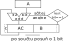
\includegraphics[width=0.7\textwidth]{multiplier-seq.pdf}

Pomalá
\end{frame}


\begin{frame}
\frametitle{Násobení celých čísel}

Rychlé násobení celých čísel Wallace tree

Motivace rychlé sečtení čtyř 64-bitových čísel
\end{frame}

\begin{frame}
\frametitle{Násobení celých čísel}

Rychlé násobení celých čísel Wallace tree
\end{frame}

\begin{frame}
\frametitle{Násobení celých čísel}

Rychlé násobení celých čísel Wallace tree

Shrnutí rychlosti násobení 64-bitových čísel
\end{frame}


\begin{frame}
\frametitle{Dělení celých čísel}

Obdoba násobení, nalezneme i zbytek po dělení

\end{frame}


\begin{frame}
\frametitle{Dělení celých čísel}

Dělička - existuje rychlejší algoritmus, ale je velmi složitý

\end{frame}


\section{Záporná čísla}
\begin{frame}
\frametitle{Reprezentace záporných čísel}
Doplněk dvou

\end{frame}

\begin{frame}
\frametitle{Opačné číslo}

Jak z X udělat -X

\end{frame}


\begin{frame}
\frametitle{Počítání se zápornými čísly}

Výhoda reprezentace doplněk dvou, nemusíme vymýšlet nové sčítání, funguje stejný algoritmus
\end{frame}

\begin{frame}
\frametitle{Odčítání}

Přičteme opačné číslo a je to.
\end{frame}

\begin{frame}
\frametitle{Přetečení}

Co se stane, když spustíte následujcí C program:

\end{frame}

\begin{frame}
\frametitle{Přetečení}

Přetečení při sčítání kladnách čísel.
\end{frame}

\begin{frame}
\frametitle{Přetečení}

Přetečení při sčítání Záporných čísel.
\end{frame}

\begin{frame}
\frametitle{Násobení a dělení}

Počítáme s absolutními hodntami a nakonec určíme znaménko výsledku podle znaménka operandů.
\end{frame}

\begin{frame}
\frametitle{Jiné reprezentace záporných čísel}

Čísla s posunutou nulou
\end{frame}

\begin{frame}
\frametitle{Počítání s posunutou nulou}

Čísla s posunutou nulou
\end{frame}


\begin{frame}
\frametitle{Jiné reprezentace záporných čísel}

Doplněk jedné

BCD formát
\end{frame}


\section{Reálná čísla}


\begin{frame}
\frametitle{Reálná čísla}

Dvojková reálná čísla

\end{frame}


\begin{frame}
\frametitle{Reálná čísla}

Čísla s pevnou destinnou čárkou

Obdoba čísel s posunutou nulou

Jednoduché sčítání odčístání, složité násobení, dělení
\end{frame}

\begin{frame}
\frametitle{Plovoucí desetinná čárka}

Plovoucí desetinná čárka, floating point numbers

Obdoba dekadického zápisu reálných čísel

\end{frame}

\begin{frame}
\frametitle{IEEE-754}

Základní definice znaménko exponent mantisa (skrytá jednička) 
\end{frame}


\begin{frame}
\frametitle{IEEE-754}

Normalizované, denormalizované čísla

Nekonečna a NaN
\end{frame}

\begin{frame}
\frametitle{IEEE-754}

Porovnání dvou reálných čísel

\end{frame}


\begin{frame}
\frametitle{IEEE-754}

Sčítání dvou reálných čísel

\end{frame}


\begin{frame}
\frametitle{IEEE-754}

Sčítání dvou reálných čísel

\end{frame}

\begin{frame}
\frametitle{IEEE-754}

Násobení dvou reálných čísel

\end{frame}

\begin{frame}
\frametitle{Bonusový bod}

Kvíz s bonusovou otázkou za tuto hodinu.

\end{frame}




\end{document}

